%-----------------------------------------------------------------------------------------------------------------------------------------------%
%	The MIT License (MIT)
%
%	Copyright (c) 2015 Jan Küster
%
%	Permission is hereby granted, free of charge, to any person obtaining a copy
%	of this software and associated documentation files (the "Software"), to deal
%	in the Software without restriction, including without limitation the rights
%	to use, copy, modify, merge, publish, distribute, sublicense, and/or sell
%	copies of the Software, and to permit persons to whom the Software is
%	furnished to do so, subject to the following conditions:
%
%	THE SOFTWARE IS PROVIDED "AS IS", WITHOUT WARRANTY OF ANY KIND, EXPRESS OR
%	IMPLIED, INCLUDING BUT NOT LIMITED TO THE WARRANTIES OF MERCHANTABILITY,
%	FITNESS FOR A PARTICULAR PURPOSE AND NONINFRINGEMENT. IN NO EVENT SHALL THE
%	AUTHORS OR COPYRIGHT HOLDERS BE LIABLE FOR ANY CLAIM, DAMAGES OR OTHER
%	LIABILITY, WHETHER IN AN ACTION OF CONTRACT, TORT OR OTHERWISE, ARISING FROM,
%	OUT OF OR IN CONNECTION WITH THE SOFTWARE OR THE USE OR OTHER DEALINGS IN
%	THE SOFTWARE.
%
%
%-----------------------------------------------------------------------------------------------------------------------------------------------%


%============================================================================%
%
%	DOCUMENT DEFINITION
%
%============================================================================%

%we use article class because we want to fully customize the page and dont use a cv template
\documentclass[10pt,A4]{article}


%----------------------------------------------------------------------------------------
%	ENCODING
%----------------------------------------------------------------------------------------

%we use utf8 since we want to build from any machine
\usepackage[utf8]{inputenc}

%----------------------------------------------------------------------------------------
%	LOGIC
%----------------------------------------------------------------------------------------

% provides \isempty test
\usepackage{xifthen}

%----------------------------------------------------------------------------------------
%	FONT
%----------------------------------------------------------------------------------------

% some tex-live fonts - choose your own

%\usepackage[defaultsans]{droidsans}
% \usepackage[default]{comfortaa}
% \usepackage{cmbright}
% \usepackage[default]{raleway}
%\usepackage{fetamont}
\usepackage{gillius}
% \usepackage[light,math]{iwona}
%\usepackage[sfdefault]{roboto}
\usepackage{lmodern}

% set font default
\renewcommand*\familydefault{\sfdefault}
\usepackage[T1]{fontenc}

% more font size definitions
\usepackage{moresize}

\usepackage{fontawesome5}

%----------------------------------------------------------------------------------------
%	PAGE LAYOUT  DEFINITIONS
%----------------------------------------------------------------------------------------

%debug page outer frames
%\usepackage{showframe}
\usepackage{paracol}

%define page styles using geometry
\usepackage[a4paper]{geometry}

% for example, change the margins to 2 inches all round
\geometry{top=1cm, bottom=0cm, left=0.5cm, right=0cm,}


%less space between header and content
\setlength{\headheight}{-5pt}


%customize entries left, center and right
%\lhead{}
%\chead{ \small{Jan Küster  $\cdot$ Consultant and Software Engineer $\cdot$  Bremen, Germany  $\cdot$  \textcolor{sectcol}{\textbf{info@jankuester.com}}  $\cdot$ +49 176 313 *** **}}
%\rhead{}


%indentation is zero
\setlength{\parindent}{0mm}

%----------------------------------------------------------------------------------------
%	TABLE /ARRAY DEFINITIONS
%----------------------------------------------------------------------------------------

%for layouting tables
\usepackage{multicol}
\usepackage{multirow}

%extended aligning of tabular cells
\usepackage{array}

\newcolumntype{x}[1]{%
>{\raggedleft\hspace{0pt}}p{#1}}%


%----------------------------------------------------------------------------------------
%	GRAPHICS DEFINITIONS
%----------------------------------------------------------------------------------------

%for header image
\usepackage{graphicx}

%for floating figures
\usepackage{wrapfig}
\usepackage{float}
%\floatstyle{boxed}
%\restylefloat{figure}

%for drawing graphics
\usepackage{tikz}
\usetikzlibrary{shapes, backgrounds,mindmap, trees, decorations.pathreplacing}


%----------------------------------------------------------------------------------------
%	Color DEFINITIONS
%----------------------------------------------------------------------------------------
\usepackage{transparent}
\usepackage{color}

%accent color
\definecolor{complcol}{RGB}{250,150,10}

%dark background color
\definecolor{bgcol}{RGB}{110,110,110}

%light background / accent color
\definecolor{softcol}{RGB}{225,225,225}

\definecolor{sectcol}{RGB}{0,120,150}


%Package for links, must be the last package used
\usepackage[hidelinks]{hyperref}

%============================================================================%
%
%
%	DEFINITIONS
%
%
%============================================================================%

%----------------------------------------------------------------------------------------
% 	ARROW GRAPHICS in Tikz
%----------------------------------------------------------------------------------------

% a six pointed arrow poiting to the left
\newcommand{\tzlarrow}{(0,0) -- (0.2,0) -- (0.3,0.2) -- (0.2,0.4) -- (0,0.4) -- (0.1,0.2) -- cycle;}

% include the left arrow into a tikz picture
% param1: fill color
%
\newcommand{\larrow}[1]
{\begin{tikzpicture}[scale=0.58]
	 \filldraw[fill=#1!100,draw=#1!100!black]  \tzlarrow
 \end{tikzpicture}
}

\newcommand{\tzlbrace}[1]
{
	\begin{tikzpicture}[ultra thick,scale=0.5,baseline={(current bounding box.base)},
	yshift=-7pt]
		\draw [decorate,#1,
			decoration = {brace}] (0,0) --  (0,1);
		\draw [decorate,#1,
			decoration = {brace}] (0.3,0) --  (0.3,1);
	\end{tikzpicture}
}
\newcommand{\tzrbrace}[1]
{
	\begin{tikzpicture}[ultra thick,scale=0.5,baseline={(current bounding box.base)},
	yshift=-7pt]
	\draw [decorate,#1,
		decoration = {brace,mirror}] (0,0) --  (0,1);
	\draw [decorate,#1,
		decoration = {brace,mirror}] (0.3,0) --  (0.3,1);
	\end{tikzpicture}
}

% a six pointed arrow poiting to the right
\newcommand{\tzrarrow}{ (0,0.2) -- (0.1,0) -- (0.3,0) -- (0.2,0.2) -- (0.3,0.4) -- (0.1,0.4) -- cycle;}

% include the right arrow into a tikz picture
% param1: fill color
%
\newcommand{\rarrow}
{
\begin{tikzpicture}[scale=0.7]
	\filldraw[fill=sectcol!100,draw=sectcol!100!black] \tzrarrow
 \end{tikzpicture}
}

%----------------------------------------------------------------------------------------
%	custom sections
%----------------------------------------------------------------------------------------

% create a coloured box with arrow and title as cv section headline
% param 1: section title
%
\newcommand{\cvsection}[1]
{
\colorbox{sectcol}{\mystrut \makebox[\linewidth][l]{
\larrow{bgcol} \hspace{-8pt} \larrow{bgcol} \hspace{-8pt} \larrow{bgcol} \textbf{\textcolor{white}{\uppercase{#1}}}\hspace{4pt}
}}\\
}

% create a coloured arrow with title as cv meta section section
% param 1: meta section title
%
\newenvironment{metasection}[1] {
    \hspace{10pt}
	\vspace{6pt}
	\begin{center}
		\textcolor{white}{\large{\uppercase{#1}}}\\
	\normalsize
	\parbox{0.7\linewidth}{\textcolor{white}	\hrule}
    }{
    \end{center}
    \hspace{10pt}
}

%----------------------------------------------------------------------------------------
%	 CV EVENT
%----------------------------------------------------------------------------------------

% creates a stretched box as cv entry headline followed by some paragraphs about
% the work you did
% param 1:	event time i.e. 2014 or 2011-2014 etc.
% param 2:	event name (what did you do?)
% param 3:	institution (where did you work / study)
% param 4:	list of paragraphs outlining your contributions, see example usage below
%
\newcommand{\cvevent}[5]
{
    \hspace{3pt}
    \parbox{1\linewidth-3pt}{
    \vspace{6pt}
    \textcolor{black}{\textbf{#2}} \hfill \textcolor{bgcol}{\textcolor{complcol}{#3}\ifthenelse{\equal{#4}{}}{}{ (#4)}, #1}
    \vspace{0pt}
    \textcolor{softcol}{\hrule}
    \vspace{6pt}
    \cvlist {#5}
    \vspace{-6pt}
    }
}

% formats a list of strings with variable length for use in `\cvevent`
% param 1: a list of strings outlining your contributions
\newcommand{\cvlist}[1] {
    \foreach \listitem in {#1}
    {
        \parbox{1\linewidth}{\larrow{softcol} \listitem\vspace{3pt}}
    }
}

% creates a stretched box as
\newcommand{\cveventmeta}[2]
{
	\mbox{\mystrut \hspace{87pt}\textit{#1}}\\
	#2
}

%----------------------------------------------------------------------------------------
% CUSTOM STRUT FOR EMPTY BOXES
%----------------------------------------- -----------------------------------------------
\newcommand{\mystrut}{\rule[-.3\baselineskip]{0pt}{\baselineskip}}


% use to vertically center content
% credits to: http://tex.stackexchange.com/questions/7219/how-to-vertically-center-two-images-next-to-each-other
\newcommand{\vcenteredinclude}[1]{\begingroup
\setbox0=\hbox{\includegraphics{#1}}%
\parbox{\wd0}{\box0}\endgroup}

% use to vertically center content
% credits to: http://tex.stackexchange.com/questions/7219/how-to-vertically-center-two-images-next-to-each-other
\newcommand*{\vcenteredhbox}[1]{\begingroup
\setbox0=\hbox{#1}\parbox{\wd0}{\box0}\endgroup}

%----------------------------------------------------------------------------------------
%	ICON-SET EMBEDDING
%----------------------------------------------------------------------------------------

% at this point we simplify our icon-embedding by simply referring to a set of png images.
% if you find a good way of including svg without conflicting with other packages you can
% replace this part
\newcommand{\icon}[3]{\makebox(#2, #2){\textcolor{#3}{\csname fa#1\endcsname}}}	%icon shortcut
\newcommand{\icontext}[4]{ 						%icon with text shortcut
	\vcenteredhbox{\icon{#1}{#2}{#4}} \vcenteredhbox{\textcolor{#4}{#3}}
}
\newcommand{\iconhref}[5]{ 						%icon with website url
    \vcenteredhbox{\icon{#1}{#2}{#5}} \href{#4}{\textcolor{#5}{#3}}
}
\newcommand{\iconemail}[5]{ 						%icon with email link
    \vcenteredhbox{\icon{#1}{#2}{#5}} \href{mailto:#4}{\textcolor{#5}{#3}}
}
\usepackage{fontspec}
\newfontfamily{\FA}[
	Path=fonts/,
]{fa-solid-900}
\newcommand{\iconnew}[3]{\makebox(#2, #2){\textcolor{#3}{\FA\symbol{"#1}}}}
\newcommand{\iconnewtext}[4]{ 						%icon with text shortcut
	\vcenteredhbox{\iconnew{#1}{#2}{#4}} \vcenteredhbox{\textcolor{#4}{#3}}
}
\newcommand{\iconnewhref}[5]{ 						%icon with website url
	\vcenteredhbox{\iconnew{#1}{#2}{#5}} \href{#4}{\textcolor{#5}{#3}}
}
\newcommand{\iconnewemail}[5]{ 						%icon with email link
	\vcenteredhbox{\iconnew{#1}{#2}{#5}} \href{mailto:Jérémie Libeau <#4>?subject=Votre profil nous intéresse !}{\textcolor{#5}{#3}}
}
\newcommand{\iconnewtel}[5]{ 						%icon with email link
	\vcenteredhbox{\iconnew{#1}{#2}{#5}} \href{tel:#3}{\textcolor{#5}{#4}}
}
\newcommand{\iconcustomtext}[4]{
	\vcenteredhbox{\makebox(#2, #2){\includegraphics[width=#2px]{#1}}} \vcenteredhbox{\textcolor{#4}{#3}}
}

%============================================================================%
%
%
%
%	DOCUMENT CONTENT
%
%
%
%============================================================================%
\begin{document}
\setlength{\columnsep}{15pt}
\columnratio{0.7}
\backgroundcolor{c[1](0pt,10000pt)}{sectcol}

\begin{paracol}{2}
\begin{leftcolumn}
%\fcolorbox{white}{white}{
%\begin{minipage}[c][0.95\textheight][t]{\linewidth}


%---------------------------------------------------------------------------------------
%	TITLE HEADLINE
%----------------------------------------------------------------------------------------
\vspace{-3pt}
% use this for multiple words like working titles etc.
%\hspace{-0.25\linewidth}\colorbox{bgcol}{\makebox[1.5\linewidth][c]{\hspace{46pt}\HUGE{\textcolor{white}{\uppercase{M.Sc. Jan Küster}} } \textcolor{sectcol}{\rule[-1mm]{1mm}{0.9cm}} \parbox[b]{5cm}{   \large{ \textcolor{white}{{IT Consultant}}}\\
% \large{ \textcolor{white}{{JS Fullstack Engineer}}}}
%}}

% use this for single words, e.g. CV or RESUME etc.
\colorbox{bgcol}{\makebox[\linewidth][c]{\HUGE{\textcolor{white}{\uppercase{Jérémie Libeau}} } \textcolor{sectcol}{\rule[-1mm]{1mm}{0.9cm}} \HUGE{\textcolor{white}{\uppercase{CV}} } }}

%----------------------------------------------------------------------------------------
%	HEADER IMAGE
%----------------------------------------------------------------------------------------


%\hspace{-1.6cm}
%\includegraphics[trim= 0 250 0 270,clip,width=1\linewidth+3.1cm]{myfoto.jpg}	%trimming relative to image size!
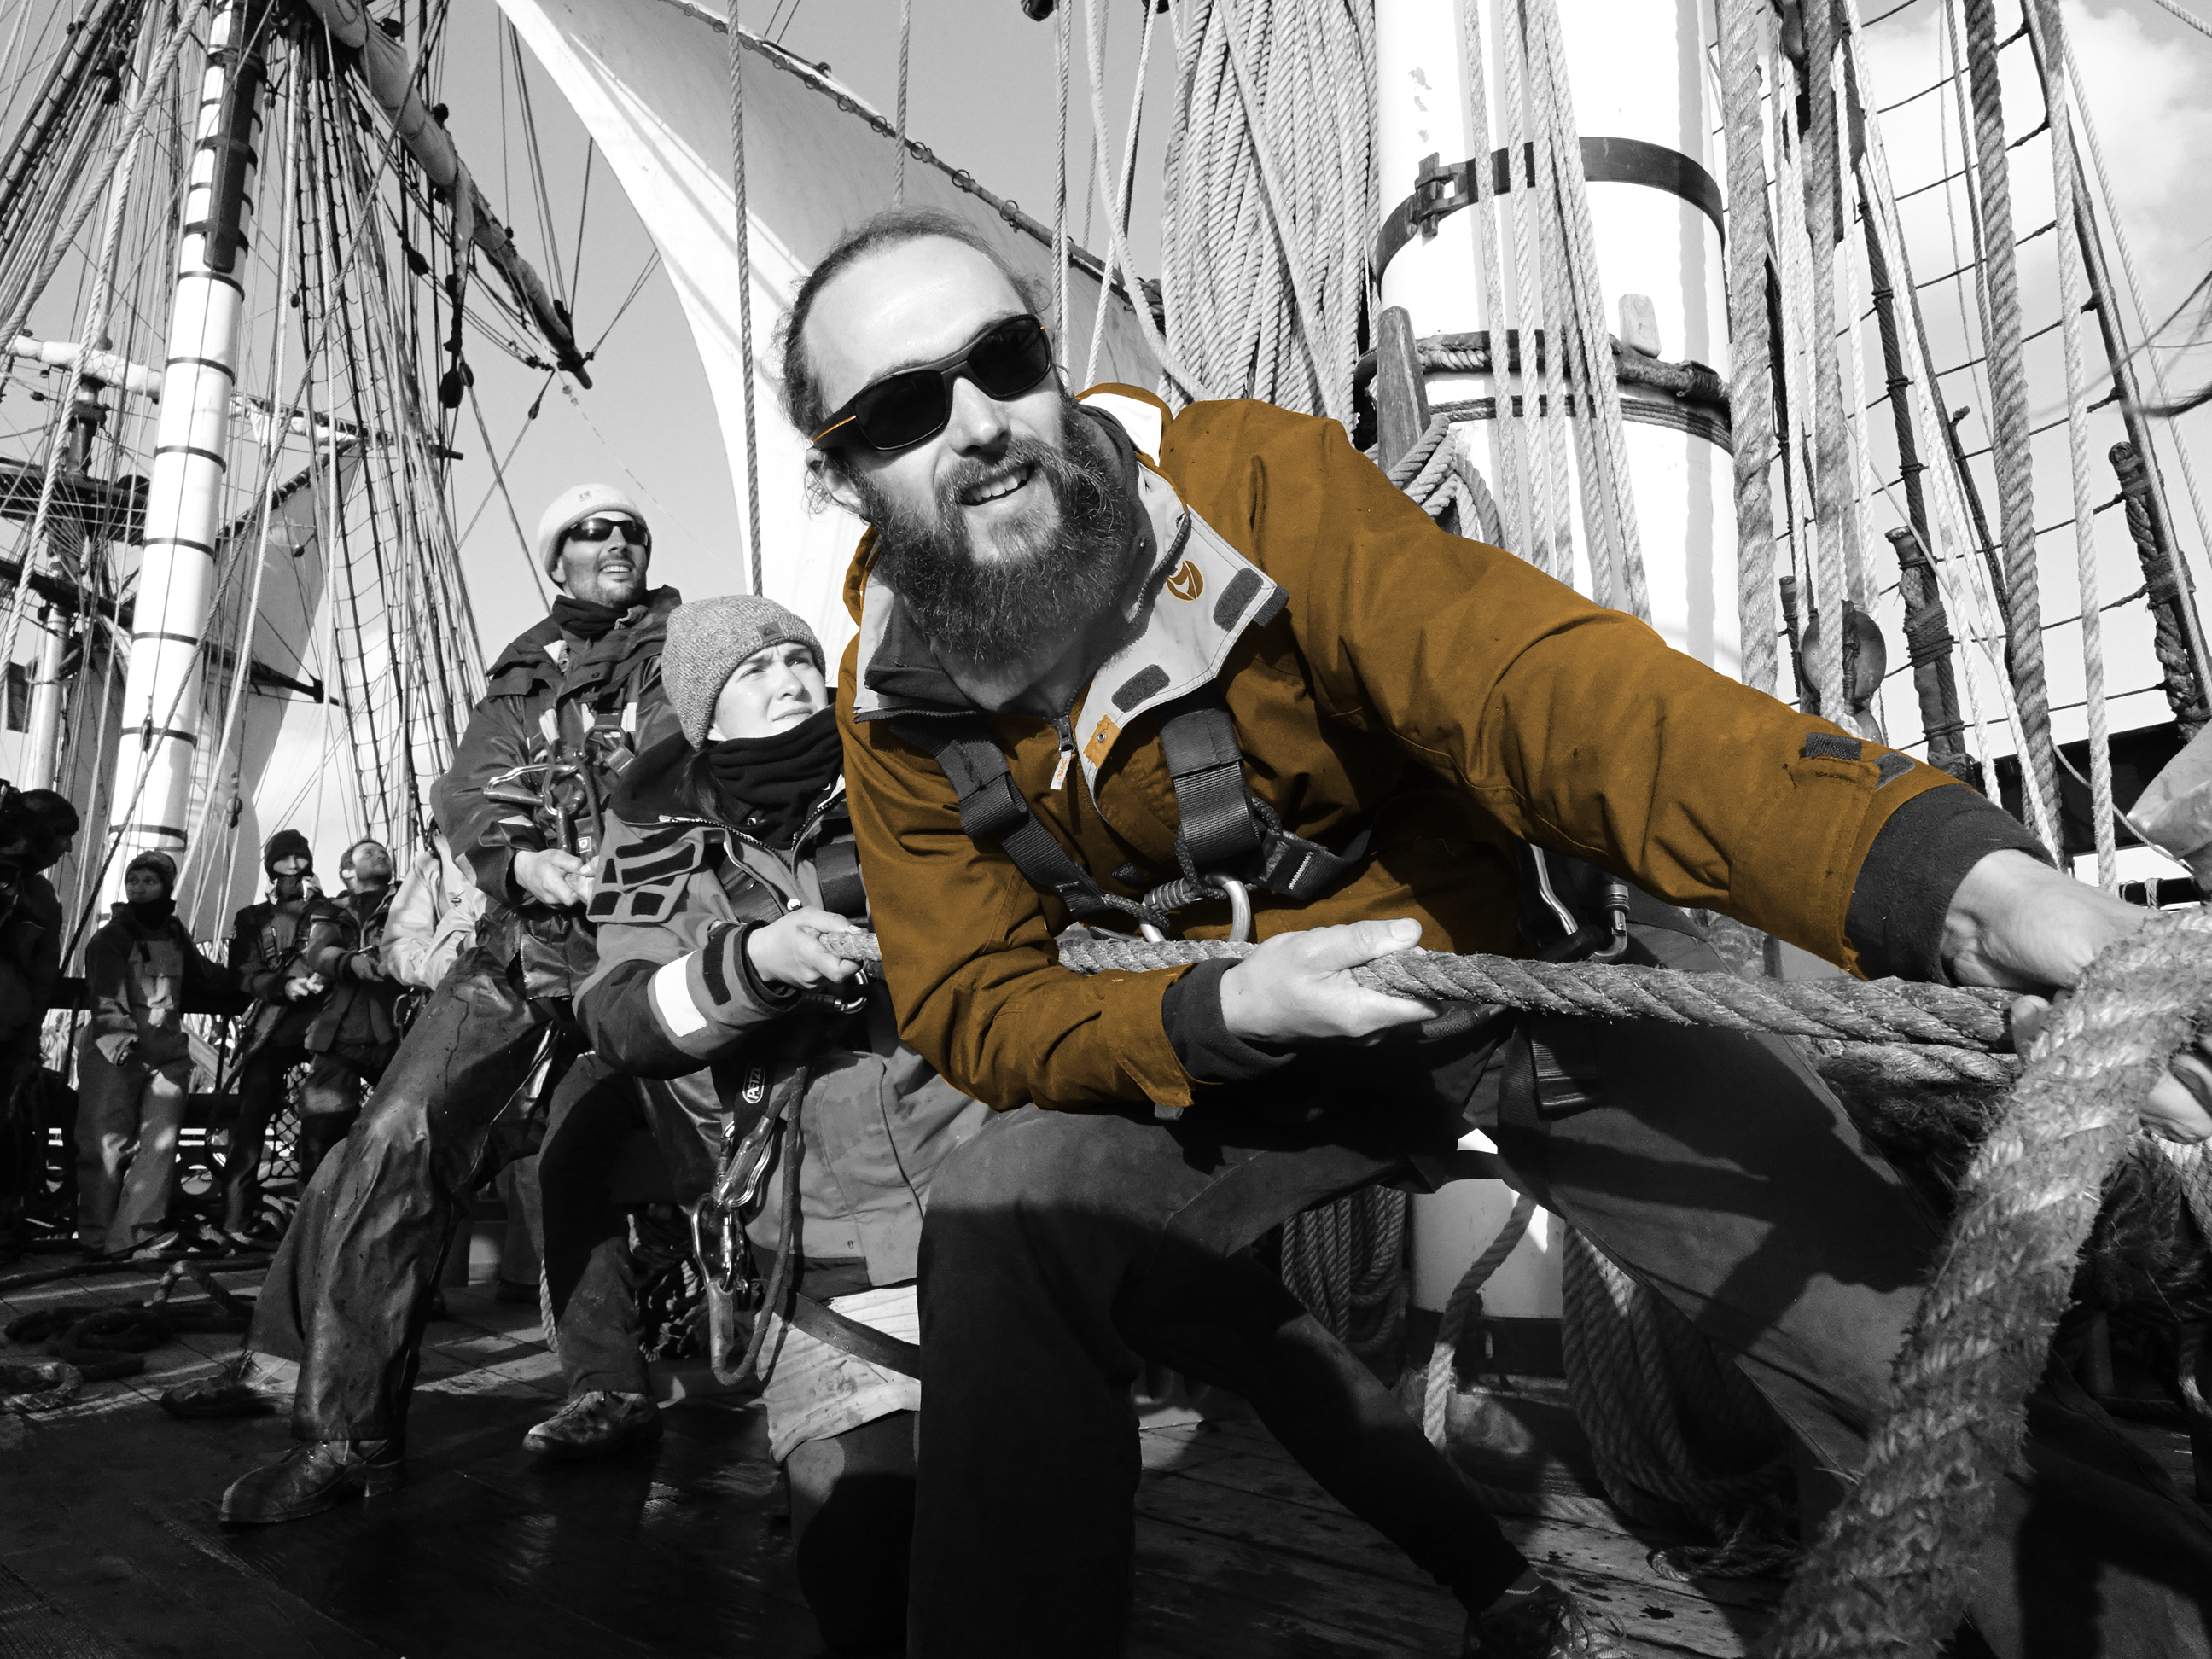
\includegraphics[trim= 100 150 0 40, clip ,width=\linewidth+5px]{images/photo.jpg}	%trimming relative to image size

%---------------------------------------------------------------------------------------
%	SUMMARY
%----------------------------------------------------------------------------------------
\transparent{0.85}%
\vspace{-180pt}
\hspace{0.59\linewidth}
\colorbox{bgcol}{
	\parbox{0.35\linewidth}{
		\transparent{1}%
		\begin{center}
		\tzlbrace{sectcol}\textcolor{white}{Discuter | Penser | Créer}\tzrbrace{sectcol}
		\end{center}
	}
}
\vspace{145pt}

%============================================================================%
%
%	CV SECTIONS AND EVENTS (MAIN CONTENT)
%
%============================================================================%

%---------------------------------------------------------------------------------------
%	STATUS
%----------------------------------------------------------------------------------------
\cvsection{Statut}

Développeur fullstack / DevOps, full remote, dans le domain du traitement des déchets

\vspace{12pt}

%---------------------------------------------------------------------------------------
%	EDUCATION SECTION
%--------------------------------------------------------------------------------------
\cvsection{Cursus}

\cvevent{2010}{Diplôme d'expert en ingénierie informatique - bac+5}{Epita}{Kremlin-Bicêtre}{
	En alternance à Siemens Mobility à Châtillon}

\cvevent{2007}{DUT Informatique}{IUT de Vannes}{}{
	Option Génie Logiciel}

\cvevent{2005}{Baccalauréat Scientifique - mention Assez Bien}{Lycée Chevrollier}{Angers}{
	Spécialisation Sciences de l'Ingénieur}

\vspace{12pt}

%---------------------------------------------------------------------------------------
%	EXPERIENCE
%----------------------------------------------------------------------------------------
\cvsection{Expériences}

\cvevent{2018/01 - maintenant}{Développeur fullstack / DevOps}{Symetri}{Rennes}{
	Backend \emph{PHP}{,} framework \emph{Symfony} et \emph{Zend}{,} base de données \emph{MSSql},
	Application mobile Android \emph{Angular + Cordova},
	Frontend web \emph{JS} et framework \emph{Angular},
	Administration de la plateforme de production cloud OBS,
	Développement de tests unitaires et fonctionnels via \emph{PHPUnit},
	Mise en place d'une plateforme d'intégration et de déploiement continu \emph{Jenkins} puis \emph{Gitlab},
	Dockerisation des applications et mise en place d'une infrastructure \emph{Kubernetes},
	Participation à la coordination projet \emph{SCRUM}}

\cvevent{2014/05 - 2017/12}{Développeur fullstack}{Avenue du Web}{Rennes}{
	Backend \emph{PHP} et framework \emph{Symfony 2}{,} base de données \emph{MySQL},
	Développement d'un système de commentaire live web{,} basé sur websocket,
	Frontend JS,
	Administration des outils de développement,
	Développement de tests unitaires et fonctionnels via \emph{PHPUnit},
	Mise en place d'une plateforme de tests automatiques \emph{Jenkins},
	Participation à la coordination projet \emph{SCRUM}}

\cvevent{2013/06 - 2014/03}{Développeur fullstack}{Outscale}{Saint-Cloud}{
	Développement et intégration de logiciels de reporting et de facturation,
	Documentation technique,
	Administration ponctuelle du SI,
	Participation à la coordination projet \emph{SCRUM}}

\cvevent{2011/08 - 2013/02}{Data Manager}{Ubisoft}{Montreuil}{
	Support technique sur les différentes consoles du marché et à venir,
	Tests de qualité sur les jeux en développement,
	Gestion de l'archivage des différentes versions des jeux,
	Gestion de l’espace de partage documentaire,
	Rédaction de documentation}

\cvevent{2011/10 - 2013/10}{Administrateur Systèmes Unix/Linux}{Siemens Mobility}{Châtillon}{
	Apprentissage de 3 ans dans le cadre du diplôme d’ingénieur expertise informatique,
	Réponse aux besoins utilisateur,
	Etude et mise en place d’un nouveau parc de machines Suse Linux,
	Supervision du data center via cacti et nagios,
	Développement d'outils d'aide à la production}

\vspace{12pt}

%---------------------------------------------------------------------------------------
%	EDUCATION SECTION
%--------------------------------------------------------------------------------------
\cvsection{Formations}

\cvevent{2017/06}{Développement web avec Symfony2}{SensioLabs}{}{
	4 jours,
	Maîtrise du framework Symfony 2}

\vspace{12pt}

\cvsection{Engagements associatifs}

\cvevent{2016 - 2018}{Membre du CA}{Association Grifon}{}{
	Grifon a pour but la promotion{,} l’utilisation et le développement d’Internet localement,
	Participe aux discutions avec les collectivités locales pour le projet d'utilisation du réseau en fibre optique de la ville et pour le projet de collecte ADSL via Rennes Métropole Télécom,
	\href{https://grifon.fr/}{grifon.fr}}

\cvevent{2016 - 2018}{Membre actif}{Fédération FDN}{}{
	La fédération FDN regroupe des Fournisseurs d'Accès à Internet associatifs se reconnaissant dans des valeurs communes : bénévolat{,} solidarité{,} fonctionnement démocratique et à but non lucratif; défense et promotion de la neutralité du Net,
	\href{https://www.ffdn.org/}{ffdn.org}}


\end{leftcolumn}

\begin{rightcolumn}

\begin{metasection}{Contact}

    \iconnewtext{F3C5}{12}{Caulnes, Bretagne}{white}\\[6pt]
	\iconnewtel{F1D8}{12}{0687463241}{06 87 46 32 41}{white}\\[6pt]
    \iconnewemail{F1D8}{12}{job@jeremielibeau.fr}{job@jeremielibeau.fr}{white}\\[6pt]
	\iconhref{Github}{12}{Github}{https://github.com/loconox/}{white}\\[6pt]

\end{metasection}

%----------------------------------------------------------------------------------------
%	META SECTION
%----------------------------------------------------------------------------------------

\begin{metasection}{Domaines}

\icontext{Code}{12}{Dévelopement Logiciel}{white}\\
\icon{Star}{12}{complcol}\icon{Star}{12}{complcol}\icon{Star}{12}{complcol}\icon{Star}{12}{complcol}\icon{Star}{12}{complcol}\icon{Star}{12}{complcol}\icon{Star}{12}{complcol}\icon{Star}{12}{complcol}\icon{Star}{12}{complcol}\icon{Star}{12}{complcol}\\[6pt]

\iconnewtext{F233}{12}{Administration Système}{white}\\
\icon{Star}{12}{complcol}\icon{Star}{12}{complcol}\icon{Star}{12}{complcol}\icon{Star}{12}{complcol}\icon{Star}{12}{complcol}\icon{Star}{12}{complcol}\icon{Star}{12}{white}\icon{Star}{12}{white}\icon{Star}{12}{white}\icon{Star}{12}{white}\\[6pt]

\iconnewtext{E533}{12}{Gestion de projet}{white}\\
\icon{Star}{12}{complcol}\icon{Star}{12}{complcol}\icon{Star}{12}{complcol}\icon{Star}{12}{complcol}\icon{Star}{12}{white}\icon{Star}{12}{white}\icon{Star}{12}{white}\icon{Star}{12}{white}\icon{Star}{12}{white}\icon{Star}{12}{white}\\[6pt]

\end{metasection}

\begin{metasection}{Technologies}

\textcolor{white}{
	\icontext{Php}{12}{PHP}{white}
	\icontext{Symfony}{12}{Symfony}{white} \\[6pt]
	\icontext{Code}{12}{Zend}{white}
	\icontext{Js}{12}{Javascript}{white} \\[6pt]
	\iconcustomtext{images/angular.png}{12}{Angular}{white}
	\icontext{Docker}{12}{Docker}{white} \\[6pt]
	\icontext{Linux}{12}{Linux}{white}
	\icontext{Cloud}{12}{Cloud}{white} \\[6pt]
}
\end{metasection}

\begin{metasection}{Outils}

\textcolor{white}{
	\iconcustomtext{images/PhpStorm.png}{12}{PhpStorm}{white}
	\icontext{Gitkraken}{12}{Gitkraken}{white}\\[6pt]
	\icontext{Terminal}{12}{Terminal}{white} \icontext{Gitlab}{12}{Gitlab}{white} \\[6pt]
    \iconnewtext{E488}{12}{Redmine}{white}
}
\end{metasection}


\begin{metasection}{OS}

    \textcolor{white}{\LARGE{\icon{Linux}{24}{white} \icon{Apple}{24}{white}  \icon{Windows}{24}{white}}}

\end{metasection}


\newpage

\begin{metasection}{Activities}

	\textcolor{white}{\LARGE{\icon{BattleNet}{24}{white} \icon{Anchor}{24}{white}  \iconnew{F86B}{24}{white}}}

\end{metasection}

\begin{metasection}{Langues}

	\textcolor{white}{Français}\\
	\icon{Star}{12}{complcol}\icon{Star}{12}{complcol}\icon{Star}{12}{complcol}\icon{Star}{12}{complcol}\icon{Star}{12}{complcol}\icon{Star}{12}{complcol}\icon{Star}{12}{complcol}\icon{Star}{12}{complcol}\icon{Star}{12}{complcol}\icon{Star}{12}{complcol}\\[6pt]

	\textcolor{white}{Anglais}\\
	\icon{Star}{12}{complcol}\icon{Star}{12}{complcol}\icon{Star}{12}{complcol}\icon{Star}{12}{complcol}\icon{Star}{12}{complcol}\icon{Star}{12}{white}\icon{Star}{12}{white}\icon{Star}{12}{white}\icon{Star}{12}{white}\icon{Star}{12}{white}\\[6pt]

	\textcolor{white}{Espagnol}\\
	\icon{Star}{12}{complcol}\icon{Star}{12}{complcol}\icon{Star}{12}{white}\icon{Star}{12}{white}\icon{Star}{12}{white}\icon{Star}{12}{white}\icon{Star}{12}{white}\icon{Star}{12}{white}\icon{Star}{12}{white}\icon{Star}{12}{white}\\[6pt]

\end{metasection}


%\end{minipage}}


%============================================================================%
%
%
%
%	DOCUMENT END
%
%
%
%============================================================================%
\end{rightcolumn}
\end{paracol}

%-------------------------------------------------------------------------------------------------
%	ARTIFICIAL FOOTER (fancy footer cannot exceed linewidth)
%--------------------------------------------------------------------------------------------------

%\null
%\vspace*{\fill}
%\hspace{-0.25\linewidth}\colorbox{bgcol}{\makebox[1.5\linewidth][c]{\mystrut \small \textcolor{white}{Coypright 2018 jkuester@uni-bremen.de} $\cdot$ \textcolor{white}{licensed under MIT license}}}\\[-6pt]

\end{document}
